\documentclass[12pt,letterpaper]{article}
\usepackage[utf8]{inputenc}
\usepackage{amsmath}
\usepackage{amsfonts}
\usepackage{amssymb}
\usepackage{cancel}
\usepackage[hmargin=2cm,vmargin=2cm]{geometry}
\usepackage{graphicx}
\usepackage{subfig}
\usepackage{setspace}
\doublespacing
\DeclareGraphicsExtensions{.pdf,.eps,.png,.jpg}

\newcommand{\proofend}{\mbox{ }\hfill$\Box$\\}
\newcommand{\pdf}[2]{\frac{\partial #1}{\partial #2}}
\newcommand{\ddf}[2]{\frac{\mathrm{d} #1}{\mathrm{d} #2}}
\newcommand{\ee}[1]{\cdot10^{#1}}
\newcommand{\eqqref}[1]{Equation \ref{#1}}

\begin{document}

{
\centering
\part*{An Electron Dispersion Compensator}
\section*{A Dispersion Compensator for Ultrafast Electron Pulses}
\section*{Untimed Pulse Compression For Electron Dispersion}
\section*{Untimed Dispersion Compensation for Ultrafast Electron Pulses}

\subsection*{Peter Hansen, Cory Baumgarten, Herman Batelaan, Martin Centurion\\
University of Nebraska-Lincoln\\
Department of Physics and Astronomy, Lincoln NE 68588\\
Email: mcenturion2@unlnotes.unl.edu}
}

\begin{abstract}
   PACS nrs.: 41.85.Ct, 41.85.-p, 42.65.Re
\end{abstract}

   \section{Introduction}

Ultrafast Electron Microscopy (UEM) and Ultrafast Electron Diffraction (UED) are techniques that are used to study the dynamics of molecular motion. 
To do this short, electron pulses are used to ``stroboscopically'' illuminate the molecules. 
Electron pulse durations are limited to about 100 fs, while molecular dynamics extends into the low femto-second regime. 
Additionally, electronic motion can currently only be investigated directly with recollision approaches. 
A technique to deliver very short electron pulses on a target may extend UEM and UED into a regime that allows all molecular motion to be studied, and may allow the study of electronic motion of arbitrary targets.

Pulsed electron sources with pulse durations below 100 fs \cite{Bat} and even at sub-cycle duration (2.7 fs at 800 nm) have been reported \cite{Kasevich,Hommelhof}.  
For these electron sources, the pulse has an appreciable energy spread of typically about 1 eV independent of energy. 
At a useful energy for UEM (100 keV) this means that the arrival time spread at a target 1 cm away from the source is a $\cancel{\text{few microseconds}}$ even with a point source pulse. 
It is clear that a technique is required that reduces the temporal spread. 
Proposals for temporal lenses call for pulsed laser beams \cite{PNAS} or pulsed RF cavities \cite{Kraus} to affect the velocity of the electrons so that they regroup at the target. 
In this paper, we discuss an alternative idea to overcome the problem.

We borrow an idea from optics, an optical dispersion compensator, and propose to use magnetic fields and a Wien filter to construct an  electron dispersion compensator. 
The differences between our electron dispersion compensator and the above mentioned solutions \cite{PNAS,Kraus} is that the electron dispersion compensator is time independent, so like the optical dispersion compensator, it does not have to be synchronized with the electron pulses. 
A drawback is that this system can at best produce a pulse width as short as the one we start with. 
However, current electron source produce pulse widths well into the regime beneficial for UED and UEM. \cite{Kraus}

\begin{figure}[tb]
   \centering
   \subfloat[Electron Dispersion Compensator]{\label{setup_e}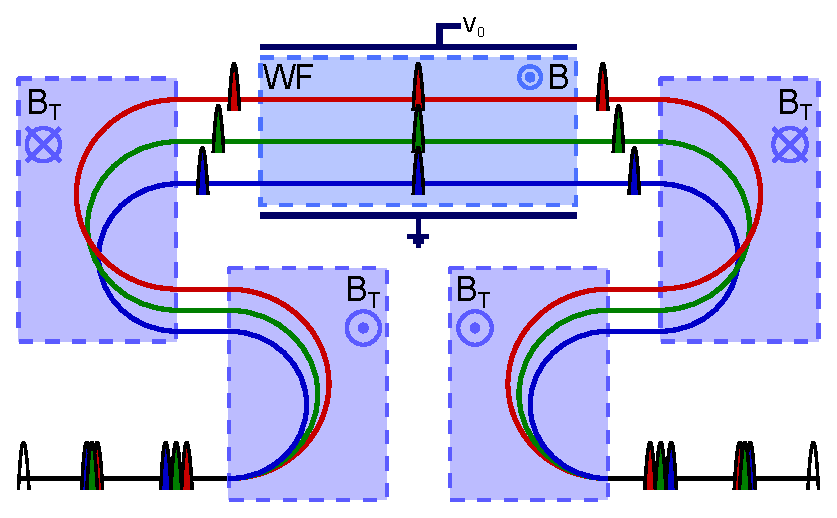
\includegraphics[width=.45\textwidth]{Setup}}
   \hspace{4mm}
   \subfloat[Optical Dispersion Compensator]{\label{setup_o}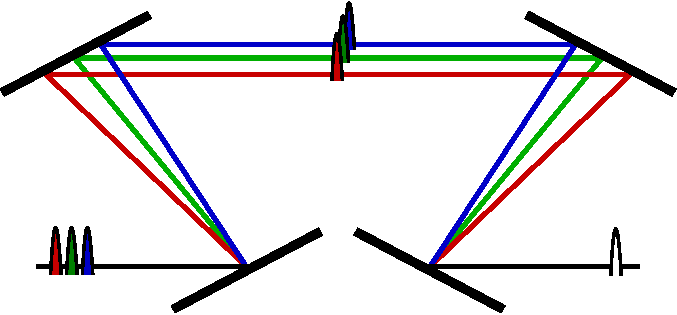
\includegraphics[width=.45\textwidth]{optical}}
   \caption{(a) Proposed setup for the electron dispersion compensator which was drawn heavly from the ideas used in an optical dispersion compensator (b).}
\end{figure}

The electron dispersion compensator (EDC), in Figure \ref{setup_e}, is modelled after the optical dispersion compensator (ODC), in Figure \ref{setup_o}.  
The first element in the optical dispersion compensator is an angled grating which disperses the light to different angles according to wavelength.  
In the EDC, the first magnetic field points perpendicular to the plane of motion and turns the electrons with a radius proportional to their velocity. 
A second angled grating in the ODC redirects the light to a path parallel to the incoming path but separated spatially by wavelength. 
Similarly, a second magnetic field turns the electrons back around, resulting in the same parallel paths, spatially separated by velocity. 
A mirror image of the two angle gratings will recombine the beam back to its original form; likewise, two magnetic fields will recombine the electron pulse. 
Since light in a vacuum has a linear dispersion relation, the phase velocity $v_{p\gamma}$ is equal to the group velocity $v_{g\gamma}$. 
An electron pulse has a quadratic dispersion relation, thus the phase velocity $v_{pe}$ is twice the group velocity $v_{ge}$. 
These relations, shown in \eqqref{eq:disp}, show that a different compensation method is needed,
\begin{align}
   \label{eq:disp}
v_{p\gamma} = v_{g\gamma}=c &\qquad  v_{pe} = 2 v_{ge} = \frac{p_e^2}{2m_e}
\end{align}

where $c$ is the speed of light, $p_e$ is the electron momentum, and $m_e$ is the electron mass. 
The compensation $\Delta t$ in the ODC is accomplished through the path length difference $\Delta l$, by $\Delta t=\Delta l/c$. 
For the EDC, $\Delta t$ depends on a velocity change $\Delta v$, so $\Delta t = l/\Delta v$ where $l$ is the path length. 
We use a Wien Filter (WF), that is, a pair of crossed magnetic and electric fields to introduce the change in velocity. 
Higher energy electrons (red paths in Figure \ref{setup_e}) enter the WF at a higher potential and are slowed down, while the lower energy electrons (blue paths in Figure \ref{setup_e}) enter at a lower potential and speed up. 
After the electrons exit the filter, they to return their initial velocity.
The higher energy electrons leave the filter behind the lower energy electrons.
As they continue to propogate the higher energy electrons will catch up to the slower ones, recreating the short pulse that was generated at the source. 

Notice the symmetry in \ref{setup_e}

\section{Theory}


\section{Simulation}

\section{Conclusion}
\end{document}

